\section{Design}
\label{s:ch5-Design}
Before diving into implementing the code, it is always imperative to have a
whiteboard and design the architecture of the tool being built. The tool that
will be made will have a single source of truth for a schema that will then be
taken and processed through the logic of the application and transformed into
structured folders containing files that represent each living part of the
source. The markdown will support framework-agnostic plug-in and integration,
meaning that any JSX framework can parse it and build HTML static files that any
browser can read. It is vital to support as many types and Scalars as possible
to consistently generate the files from any schema, regarding their complex tree
structure and the scalars used by the producer. The diagram below visually
explores the solution that will be chased for the end goal.

\begin{figure}[H]
  \centering
  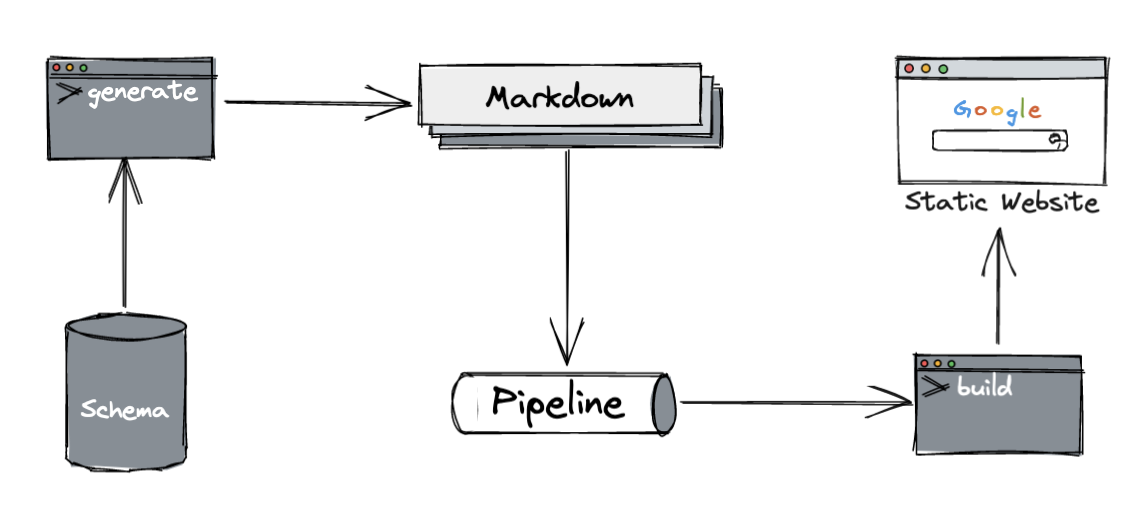
\includegraphics[width=0.7\textwidth]{figures/architecture}
  \caption{High-Level Architecture}
  \label{f:ch5-architecture}
\end{figure}

\section{Proof of Concept}
\label{s:Proof of Concept}
This section will discuss the first iteration of the project as Proof of Concept
(PoC). This will be the initial implementation stage of the project used for
discovery and testing. The PoC is a software development methodology that helps
the project developers implement the initial logic and validate their hypothesis
on the project's feasibility. This specific PoC will be coded in JavaScript
using Node as a backend runtime. In a perfect world, the tool should be written
using a more robust programming language and ecosystem such as Scala to have the
advantage of an effectful, high-performance in pure functional programming. This
would massively improve concurrency with the use of IO, which facilitates Fibers
as a replacement for native OS threads and allows for the benefit of millions of
concurrent processes without the need for a thread manager. In this use case,
the PoC is using JavaScript to keep things simple, without looking too much at
the performances that it would have in a production environment as it will be
only used to demonstrate how feasible the project is. Since JavaScript does not
support the concept of template literals, a templating language named Handlebars
will be used to generate the inside structure of the markdown files. Handlebars
use expressions that are evaluated and replaced with the evaluation results. An
example of this can be seen below.

\begin{figure}[H]
  \centering
  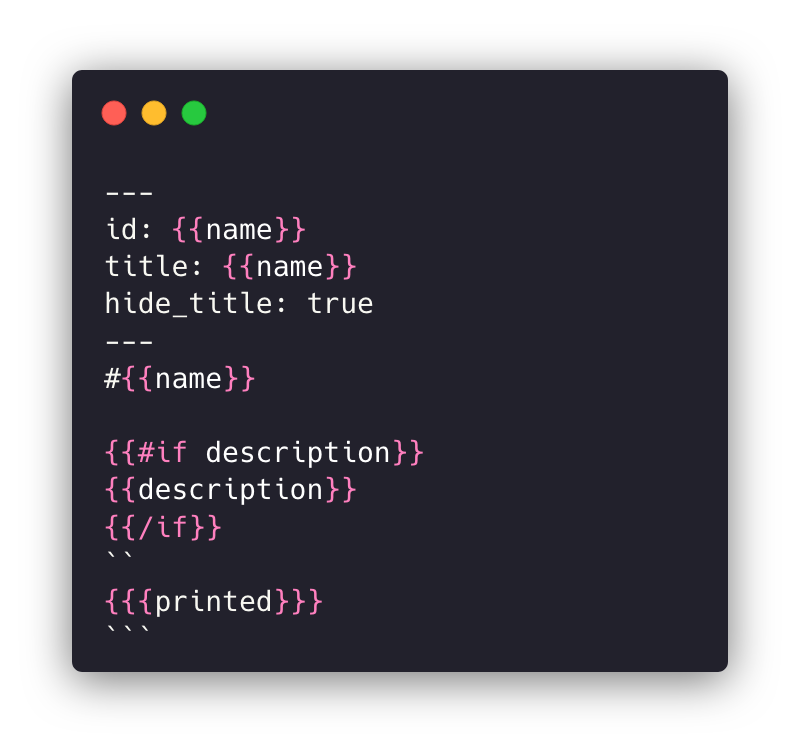
\includegraphics[width=0.5\textwidth]{figures/code/handlebars.png}
  \caption{Handlebars Template Language}
  \label{f:ch5-handlebars-template-language}
\end{figure}

The imports for the PoC will be kept at the very minimal. Below is shown
the start of the index file with the imported tools to complete and reach the
end goal.
\
\begin{figure}[H]
  \centering
  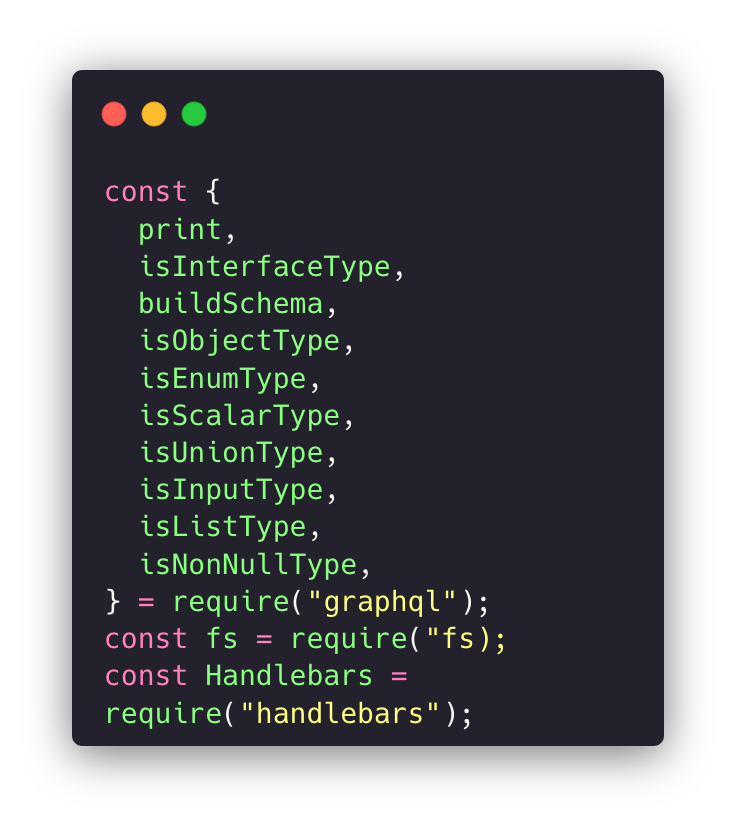
\includegraphics[width=0.5\textwidth]{figures/code/poc-imports.png}
  \caption{PoC Imports}
  \label{f:ch5-poc-imports}
\end{figure}

In order for it to work, we need to install the GraphQL library and import
all the type guards that are implemented in it to be able to check the types
while navigating in the complex nested structure of the Abstract Syntax Tree (AST)
generated by the reading the schema given in the folder. An example on how the
type guards are implemented is shown in the image below.

\begin{figure}[H]
  \centering
  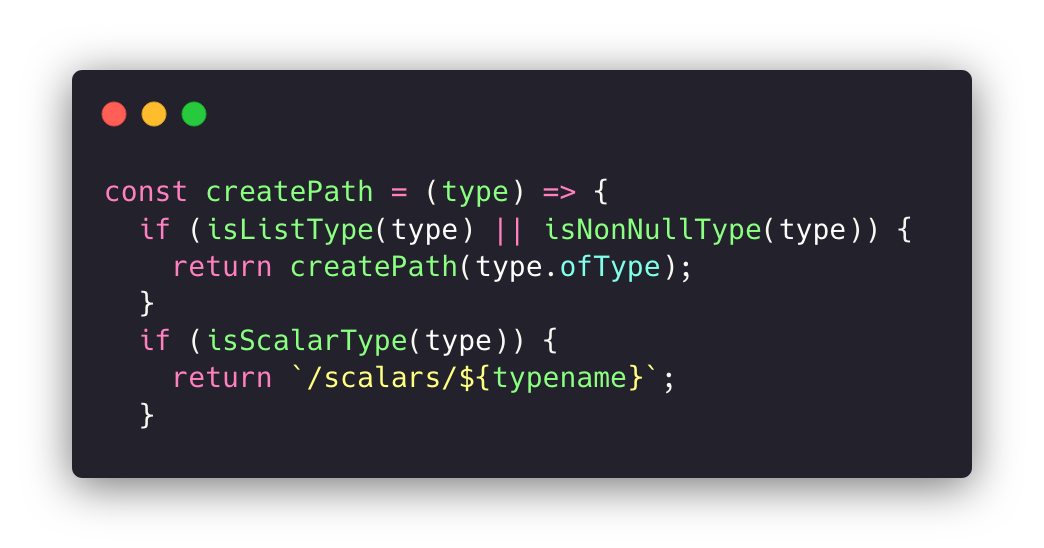
\includegraphics[width=0.5\textwidth]{figures/code/poc-type-guards.png}
  \caption{PoC Type Guards}
  \label{f:ch5-poc-type-guards}
\end{figure}

Since in the markdown file, there are places where it would be nice to have
hyperlinks that point the user to the right page when navigating the
relationship between the fields, there is a need of the type guards to be able
to place the right path into the object of a specific formatted data structure
used to group the data. An example of the object related to the image above is
shown below.

\begin{figure}[H]
  \centering
  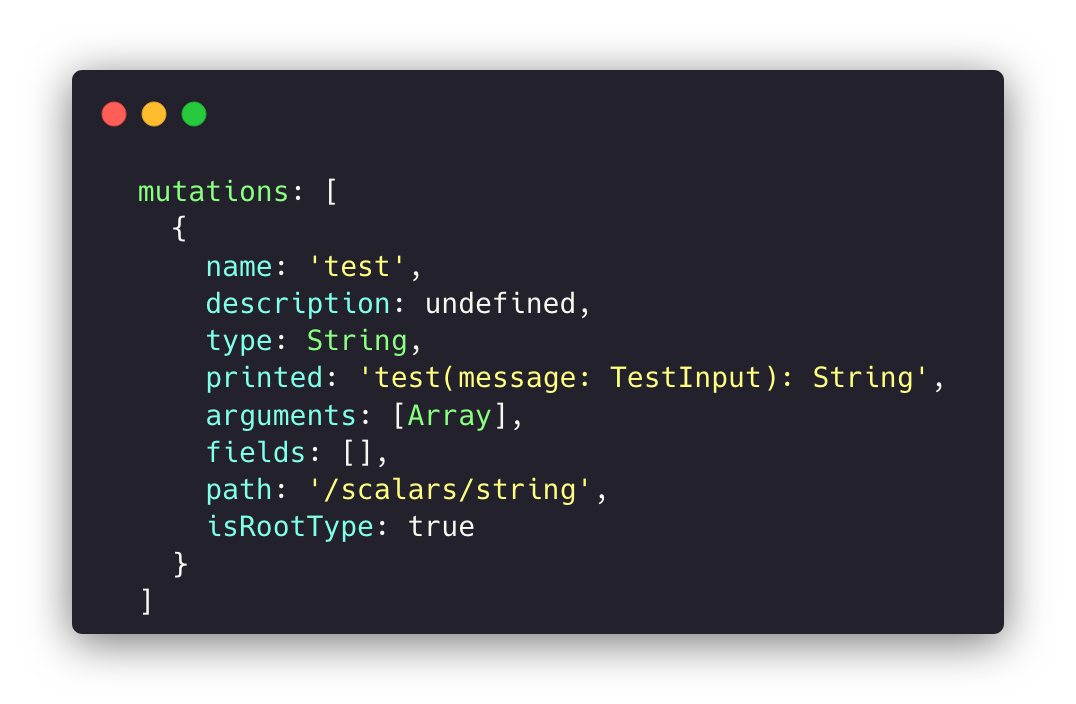
\includegraphics[width=0.5\textwidth]{figures/code/poc-scalar-type.png}
  \caption{PoC Scalar Path}
  \label{f:ch5-poc-scalar-path}
\end{figure}

As shown in the image above, the field has a type of \texttt{String} and the
path to the scalar is \texttt{/scalar/string}. The type guard is implemented as
a way to recursively navigate the AST and find the right path to the each
specific hyperlink case.

\begin{figure}[H]
  \centering
  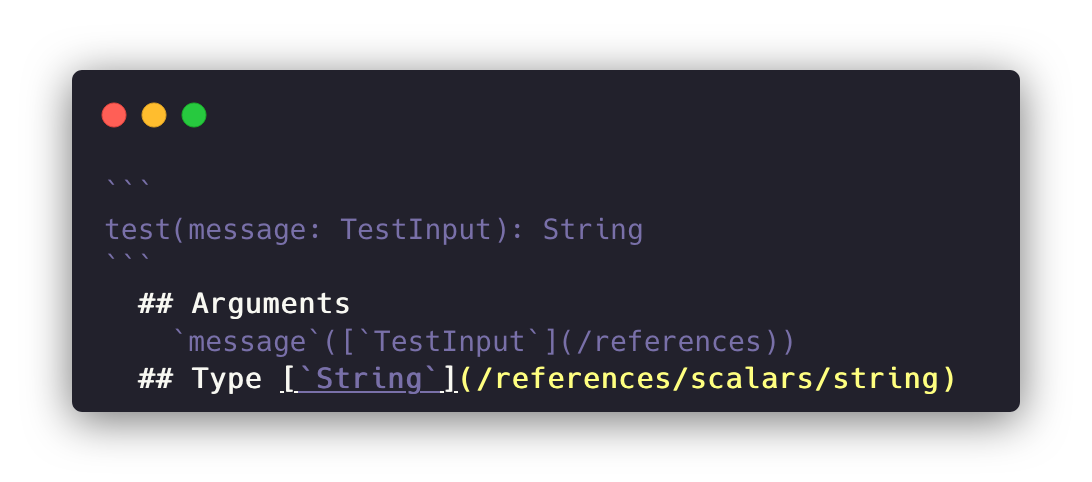
\includegraphics[width=0.5\textwidth]{figures/code/poc-generated-path.png}
  \caption{PoC Scalar Path Markdown}
  \label{f:ch5-poc-scalar-path-markdown}
\end{figure}

The image above shows the exact same mutation but in a generated markdown format,
completely done by the tool.

In order to have a great structure of the data we are going to manipulate for
the generation, a special lambda function has been created which return an object
with all the properties each type has to offer, it goes and traverse the AST and
places the information in the right properties available for later use.

\begin{figure}[H]
  \centering
  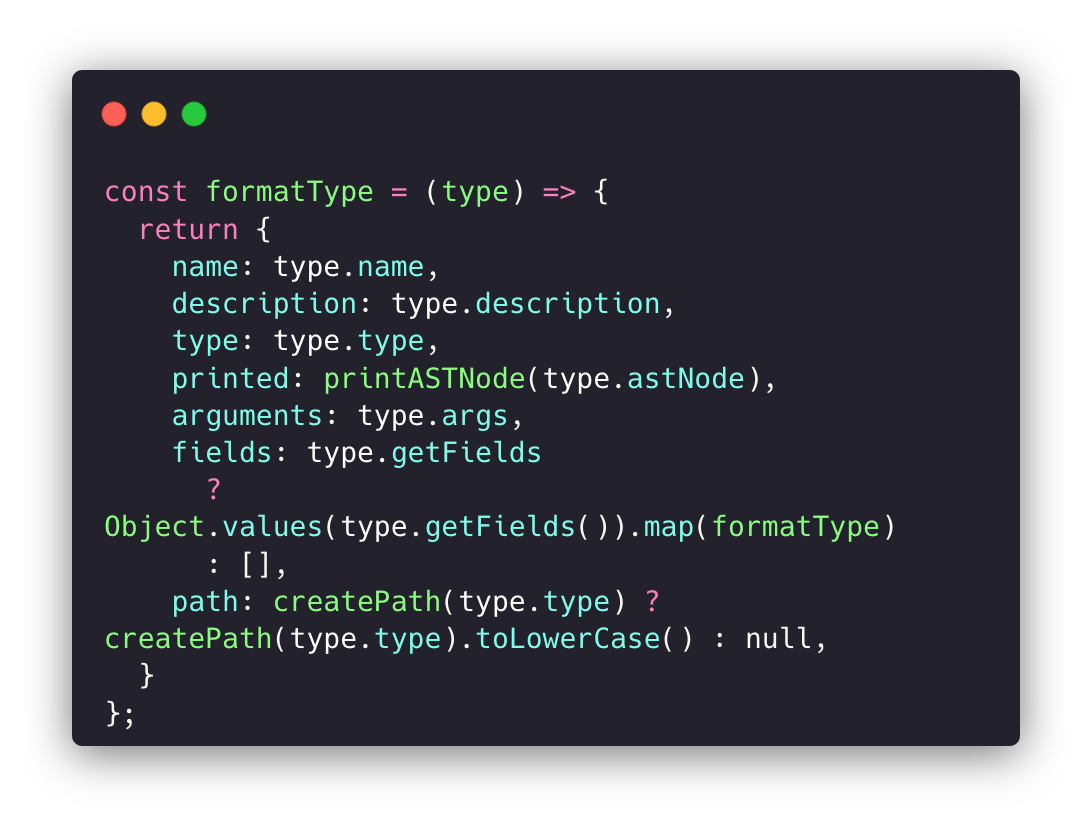
\includegraphics[width=0.5\textwidth]{figures/code/poc-format-type.png}
  \caption{PoC Format Type Lambda Function}
  \label{f:ch5-poc-format-type-lambda-function}
\end{figure}

It is important to note there is another function operating in the body formatType
which is used to pull out the printed version taken from the schema. This is
useful to have so that the documentation can have an original representation of
the piece of schema that is being discussed. The image below represent the function
written to achieve the printed version of the schema in the formatted structure.

\begin{figure}[H]
  \centering
  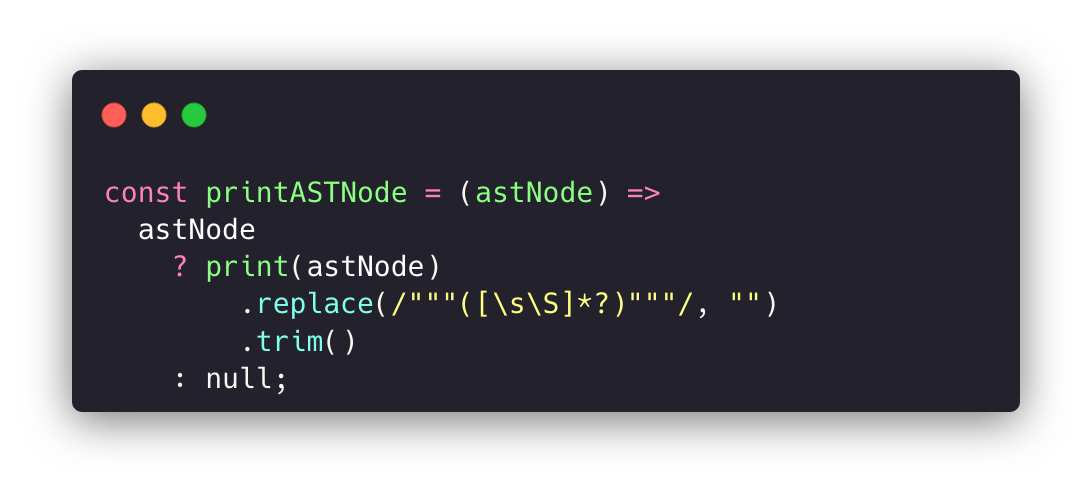
\includegraphics[width=0.5\textwidth]{figures/code/poc-print-ast.png}
  \caption{PoC Print AST Node}
  \label{f:ch5-poc-print-ast-node}
\end{figure}

It is again a lambda function that is used to traverse the AST till it reaches a
specific node and then surgically extract the printed version of it, making sure
it doesn't have any unwanted literal strings, characters or whitespace in it, so
that it can directly be used without any further manipulation in the templating
system previously described.

One of the last pieces of the puzzle is a wrapper that groups all types in a
last and single object, done used the previously described functions recursively
for any type in the AST. This prints out a massive object that is then used in a
nested loop to again recursively generate the markdown files for each type, while
accessing the Handlebars templating for valuating the expressions.

The structure of the final, but empty, data structure is as shown below.


\begin{figure}[H]
  \centering
  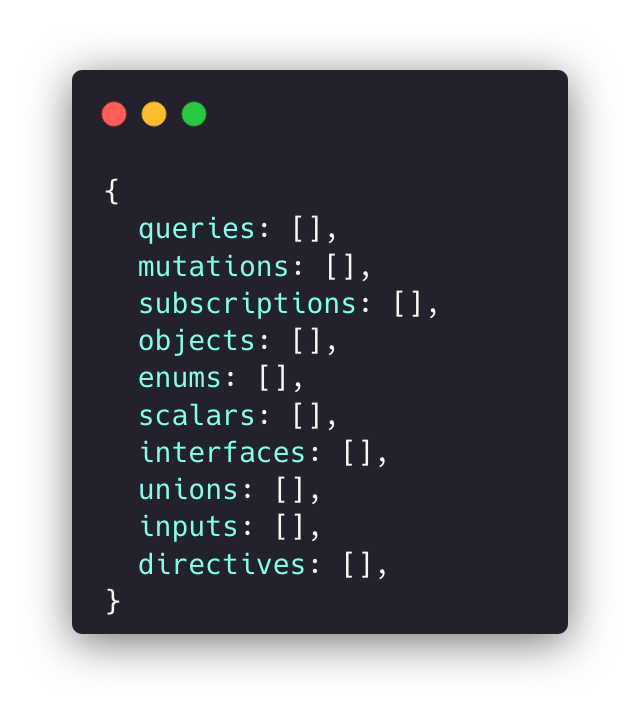
\includegraphics[width=0.5\textwidth]{figures/code/poc-empty-structure.png}
  \caption{PoC Empty Structure}
  \label{f:ch5-poc-empty-structure}
\end{figure}

The structure is being shown as empty because it would be too much to show in a
single image. In order to facilitate the understanding, below also an image
representing a single type with its full array structure.

\begin{figure}[H]
  \centering
  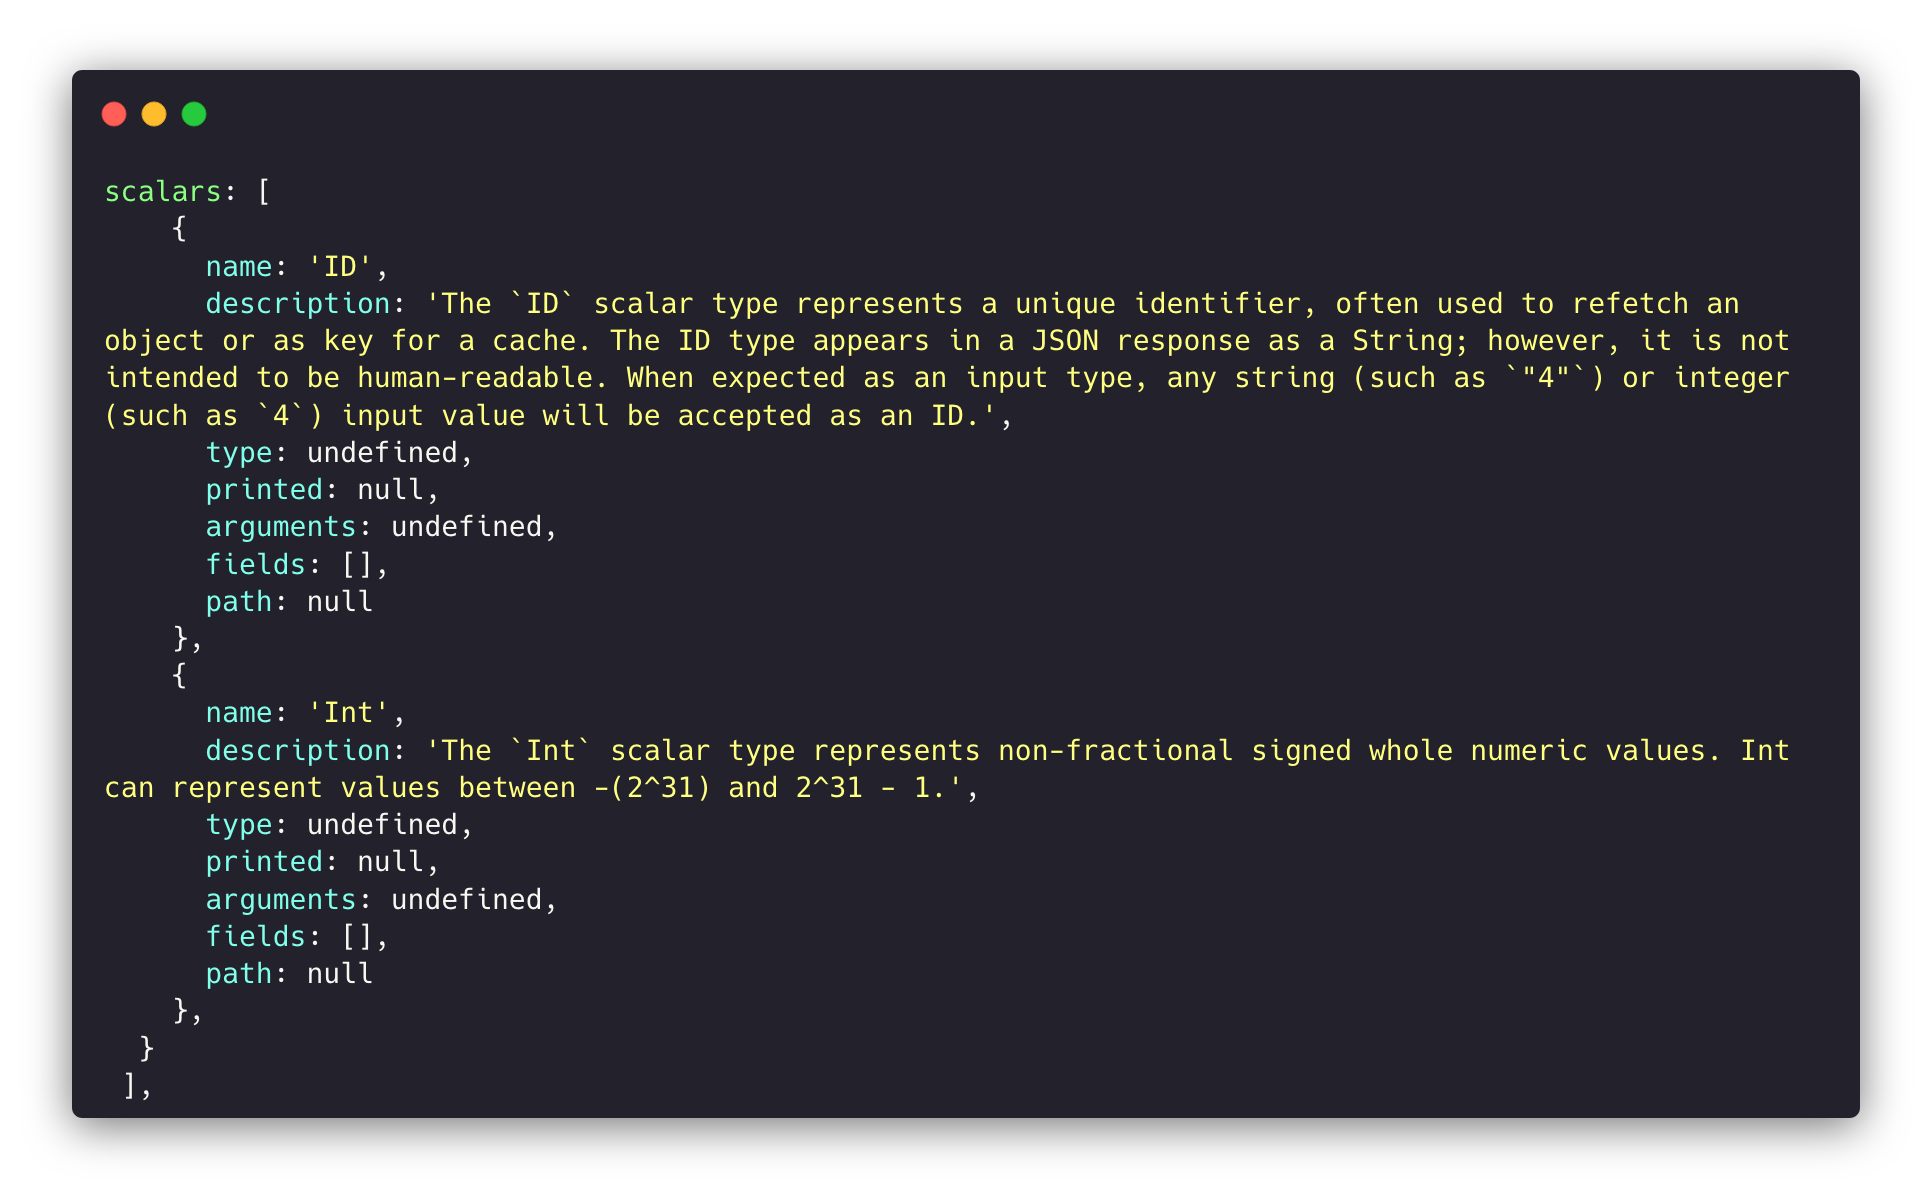
\includegraphics[width=0.8\textwidth]{figures/code/poc-full-structure.png}
  \caption{PoC Full Structure}
  \label{f:ch5-poc-full-structure}
\end{figure}

And as previosuly mentioned, the final structure is then used in a nested
function shown below.

\begin{figure}[H]
  \centering
  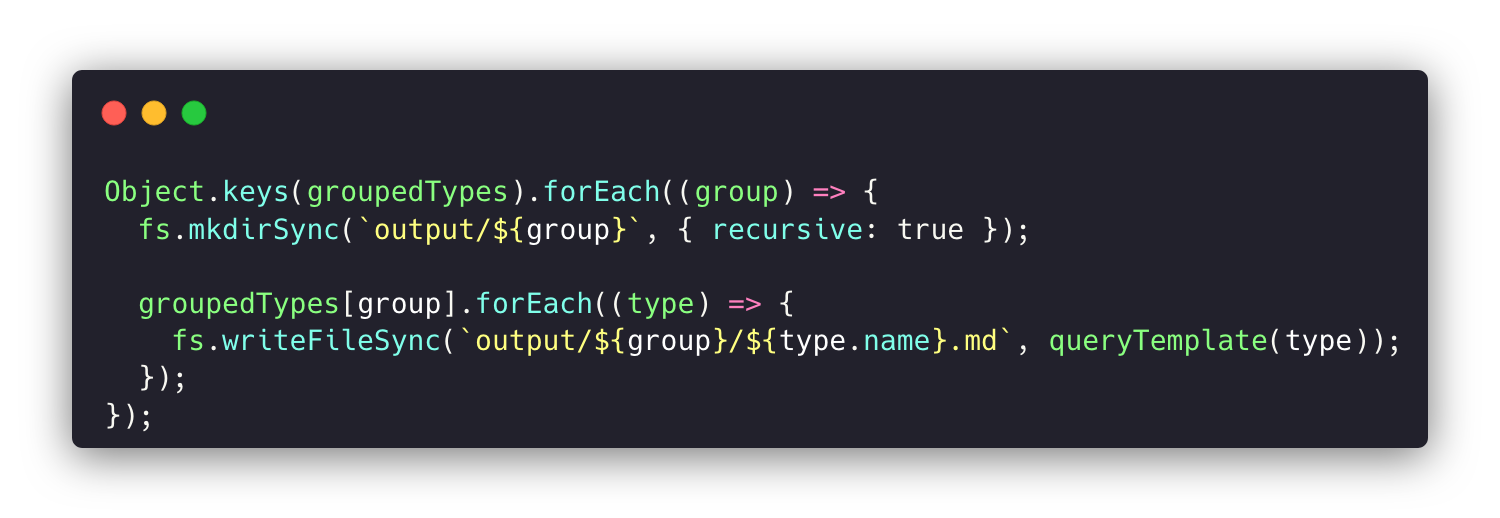
\includegraphics[width=0.8\textwidth]{figures/code/poc-nested-function.png}
  \caption{PoC Nested Loop}
  \label{f:ch5-poc-nested-loop}
\end{figure}

The nested loop makes sure that all the types are accounted for and uses the
templating system to generate the markdown files for each type.

The final output is an output folder with all the markdown files generated, and
the goal of the PoC has been validated and the code is ready to be used and
refactored for better improvements and use cases.

\begin{figure}[H]
  \centering
  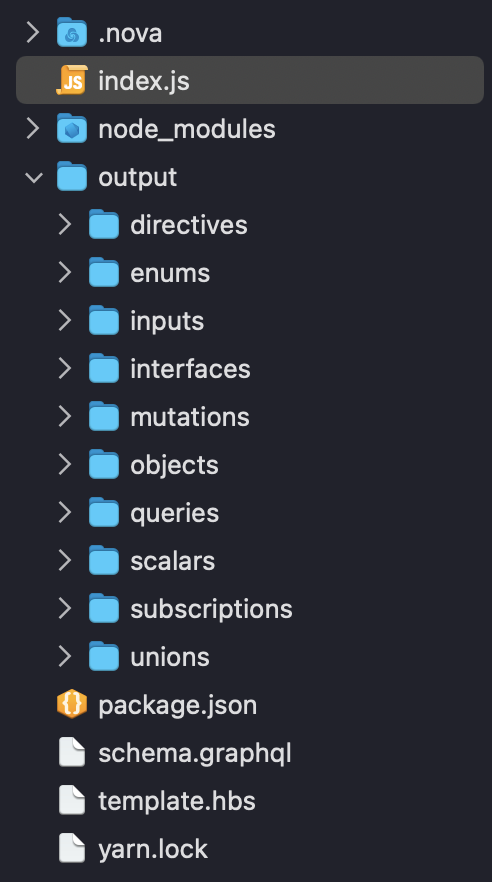
\includegraphics[width=0.3\textwidth]{figures/folders}
  \caption{PoC Output Folder}
  \label{f:ch5-poc-output-folder}
\end{figure}

Each folder has multiple md files that can be used by any framework that can
parse the markdown files and build static generated pages in HTML.

Now that the proof of concept has been completed and resulted in a successfull
experiment, the next step is to refactor the code and removing unnecessary steps
such as Handlebars templating, which will be redundant with TypeScript. It is
always good to keep the dependencies as minimum as possible in order to keep the
code clean and easy to maintain. Easy to maintain because deprecation of
functionalities are always behind the corner and it means that the code needs to
be migrated to a new version of the library which would require time, effort and
money.

\section{Refactoring}
\label{s:Refactoring}
For the same reasons explained before, the code will be then refactored in
TypeScript removes the templating system and utilises the one in-built with the
language. The template literals types will produce the same result shown and
achieved in the JavaScript PoC, making it much more succinct, readable and
powerful as the code will not be decoupled in different files and folders. It
will also keep the code much more DRY with a single source of truth, which the
language itself tries to doctrine.

\section{Frontend}
\label{s:Frontend}
In this part I will show how I produced the frontend part that generates the
website.

\section{Version Control System}
\label{s:Version-Control-System}
GitHub etc

